\documentclass{article}

\usepackage[spanish]{babel}
\usepackage[utf8]{inputenc}
\usepackage[font=footnotesize,labelfont=bf]{caption}
\usepackage{float}
\usepackage{graphicx}
\graphicspath{{images/}}

\title{Trabajo Practico 2: Universal Asynchronous Receiver Transmitter}
\author{Perez, Federico\\
        \texttt{perezfederico@unc.edu.ar}
        \and 
        Sardoy, Juan Manuel\\
        \texttt{jmsardoy@gmail.com}
        }
\begin{document}

\maketitle	
\begin{center}
    
\includegraphics[scale=2]{unc-logo}
\end{center}
\newpage
\section{Descripción del trabajo}

El siguiente trabajo consiste en la implementación práctica de un módulo completamente
funcional del protocolo UART o "Universal Asynchronous Receiver-Transmitter. \\
Como su nombre lo especifica, se trata de un protocolo asíncrono y \textit{full-duplex}
pero de facil uso e implementación dado su simplicidad.\\
La arquitectura completa del trabajo de aplicación será aproximadamente en siguiente:

\begin{figure}[H]
    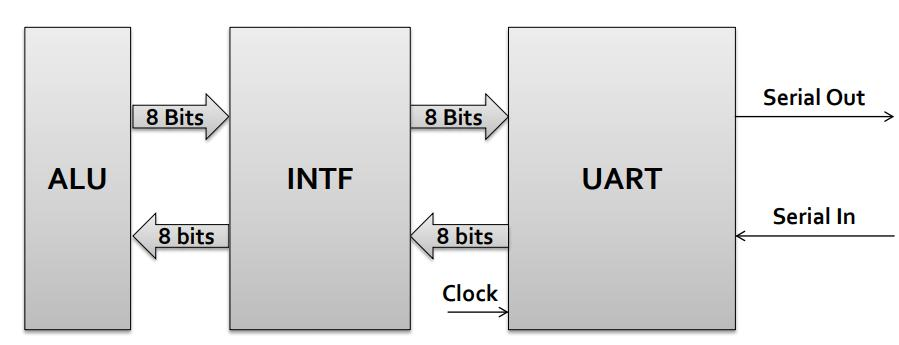
\includegraphics[scale=0.5]{arch}
    \caption{\textit{Diagrama de la arquitectura básica del proyecto}}
\end{figure}

\indent A fines prácticos y demostrativos, dicho módulo UART se conectará mediante un 
módulo que actuará de interfaz, a una \textit{Unidad Aritmetico Lógica} o ALU.
Dicho módulo interfaz contendrá lógica que permitirá procesar instrucciones y argumentos recibidos
por el módulo RX del UART, enviarlos a la ALU para su resolución, y reenviarlos por el módulo TX 
nuevamente hacia el solicitante del cálculo. \\
\indent Como usuario de dicho sistema, conectaremos el puerto USB de una computadora, y con un convertidor
\textit{USB-UART}, se enviarán las instrucciones y argumentos requeridos. Para dicho fin, además se 
desarrollará algún tipo de software que haga uso del hardware convertidor, y facilite el envío de instrucciones
y la recepción de los resultados calculados en la ALU.\\ 

\newpage
\section{Implementación}

\newpage
\section{Protocolo UART}
\indent Este protocolo, como se ha explicado anteriormente, es bastante simple. El siguiente diagrama muestra los 
datagramas básicos de una comunicación UART.

\begin{figure}[H]
    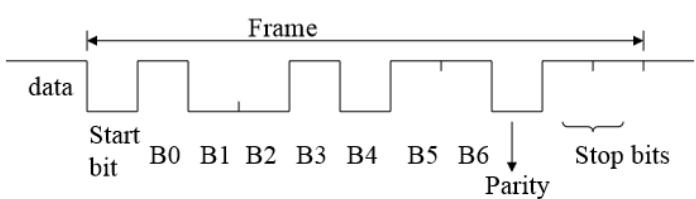
\includegraphics[scale=0.5]{protocol}
    \caption{\textit{Diagrama del datagrama del protocolo UART}}
\end{figure}

\subsection{Módulo RX}
\indent El módulo RX o receptor es el encargado de detectar el comienzo de la transmisión por el pin de recepción,
de interpretar los datos, y exponerlo por el bus de salida. Típicamente el bus de salida, y el largo de los datos recibidos
es de un \textit{byte} o 8 \textit{bits}.
\indent Como se verá también en la implementación del módulo TX, es 

\subsection{Módulo TX}



\subsection{Módulo Interface}

	

\newpage
\section{Simulación}

\end{document}
